\subsection{Quantização Vetorial}

\begin{frame}[allowframebreaks]
  \frametitle{Quantização Vetorial}
  Utilizamos a quantização vetorial em casos em que o sinal de entrada já é um sinal digital
  e queremos obter uma representação comprimida da informação origial (em geral, representando
  os dados originais através de um \textit{codebook}).

  \vspace{1cm}
  Considere uma variável aleatória $X$ que assumule valores $x \in \mathcal{X} \subseteq \mathit{R}$,
  e $\mathcal{X}^n \subseteq \mathit{R}^n$ o conjunto de vetores $\mathbf{x} = (x_1, x_2, \ldots, x_n) \in \mathit{R}^n$.

  \framebreak

  Uma quantização vetorial é um mapeamento $Q$  de vetores de entrada $\mathbf{x} = (x_1, x_2, \ldots, x_n )$,
  onde $\mathbf{x} \in \mathcal{X}^n$, nos valores $\mathbf{y} = (y_1 , y_2 , \ldots , y_n ) \in \mathcal{X}^n$
  mais próximos (com relação a alguma medida de distorção), onde $\mathbf{y} \in \mathcal{Y} \subseteq \mathcal{X}^n$,
  sendo $\mathcal{Y} = \{y_1 , y_2 , \ldots, y_M\}$, um subconjunto constituído por $M$ elementos em $\mathcal{X}^n$.
  O parâmetro $n$ indica a dimensionalidade dos dados e do quantizador. O conujunto de aproximação $\mathcal{Y}$ 
  é chamado de \textit{codebook}.

  \vspace{3em}
  Para se projetar um quantizador, devemos dividir o domínio $\mathcal{X}^n$ em $M$ áreas ou células $S_i$,
  $i = 1, 2, \ldots, M$, de forma que $\bigcup_i S_i = \mathcal{X}^n$, $S_i \cap S_j = \emptyset$, $i \neq j$,
  e $y_i \in S_i$.
\end{frame}


\begin{frame}[allowframebreaks]
  \frametitle{Erro de quantização médio}
  O erro de quantização esperado de um quantizador é dado por
  \begin{equation}
  D_n(Q) = E \{ d(\mathbf{x},Q(\mathbf{x})) \}
  \end{equation}

  Utilizando a distância Euclideana normalizada como métrica
  \begin{eqnarray}
  d(\mathbf{x},\mathbf{y}) &=& \frac{1}{n} d^2_E(\mathbf{x},\mathbf{y}) \nonumber \\
                           &=& \frac{1}{n} (\mathbf{x} - \mathbf{y}) (\mathbf{x} - \mathbf{y})^T \nonumber \\
                           &=& \frac{1}{n} \sum_{i=1}^n (x_i - y_i)^2 = \frac{1}{n} \Vert \mathbf{x} - \mathbf{y} \Vert^2
  \end{eqnarray}
  teremos
  \vspace{-1ex}
  \begin{equation}
  D_n (Q) = \frac{1}{n} E \{ \Vert \mathbf{x} - Q(\mathbf{x}) \Vert^2 \} = \frac{1}{n} \sum_{i=1}^M  E \{ \Vert \mathbf{x} - \mathbf{y_i} \Vert^2 \} .
  \label{eq:avg_quant_error}
  \end{equation}
 
  \framebreak
  Considere que a pdf n-dimensional dos dados, $f(\mathbf{x})$, sobre o conjunto $\mathcal{X}^n$ seja conhecida, 
  então a Equação \ref{eq:avg_quant_error} assume a forma 
  \begin{equation}
  D_n (Q) = \frac{1}{n} \sum_{i=1}^M \int_{S_i} f(\mathbf{x}) \Vert \mathbf{x} - \mathbf{y_i} \Vert^2 \mathrm{d}\mathbf{x} ,
  \end{equation}
  e a probabilidade do vetor de representação $\mathbf{y_i}$ é dada por
  \begin{equation}
  P(\mathbf{y_i}) = \int_{S_i} f(\mathbf{x}) \mathrm{d}\mathbf{x} .
  \end{equation}
\end{frame} 


\begin{frame}%[allowframebreaks]
  \frametitle{Taxa de quantização}
  A taxa de quantização $R$ é o número de bits necessários para representar o vetor $\mathbf{x}$
  (utilizando vetores de \textit{codebook} de tamanho $M$) por dimensão, $n$. Para um quantizador com taxa fixa
  (em que cada símbolo é codificado por palavras de mesmo tamanho em um dado \textit{codebook}), 
  a taxa é dada por
  \begin{equation}
  R = \frac{\log_2 M}{n} \textmd{ bits/amostra}.
  \end{equation}

  Para um quantizador de taxa variável, a taxa estará limitada pela entropia, ou seja,
  \begin{equation}
  R \geq - \frac{1}{n} \sum_{i=1}^M P(\mathbf{y_i}) \log_2 P(\mathbf{y_i}) \textmd{ bits/amostra}.
  \end{equation}
\end{frame}

\begin{frame}[allowframebreaks]
  \frametitle{Quantização vetorial}
  As células criadas por um quantizador vetorial em $n$-dimensões são regiões de Voronoi.

  O caso especial em que o \textit{codebook} gera uma estrutura regular é chamado 
  de quantizador vetorial em treliça (\textit{lattice vector quantizers}).

  \begin{figure}[h!]
  \centering
  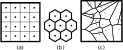
\includegraphics[width=0.6\textwidth]{images/lattice.pdf}
  \caption{Diagramas de Voronoi. Estruturas em treliça em (a) e (b).}
  \label{fig:lattice}
  \end{figure} 
\end{frame}

\begin{frame}%[allowframebreaks]
  \frametitle{Exemplo Quantização - GNU Octave}
  \centering
  \includegraphics[width=0.4\textwidth]{images/qrcode-jupyter-quantizacao.pdf}

  \url{https://nbviewer.jupyter.org/github/leolca/notebooks/blob/master/aev/quantization.ipynb}
\end{frame} 


\begin{frame}%[allowframebreaks]
  \frametitle{Exemplos de utilização}
  A quantização vetorial é utilizada em
  \begin{itemize}
  \item Video codecs: Cinepak, Sorenson codec, Indeo, VQA (utilizada em jogos)
  \item Audio codecs: CELP, G.729, TwinVQ, Ogg Vorbis, AMR-WB+, DTS
  \end{itemize}
\end{frame}


